% One incoming text, two ways to handle it. Top: an illustration of an agent with no gate (not one
% of the tested systems). Bottom: Plan B. Both lanes share three columns so the comparison reads
% column by column.
\documentclass[border=3pt]{standalone}
% Shared style of every Plan B figure (the deck, the poster and the documentation).
% Type is near-black and grey on white. UMB blue is the brand and the system. One warm accent
% marks tension only (the incoming message, the clock). Green marks only an accepted receipt or
% a met run. Square corners, thin rules, no shadows, no gradients.
\usepackage[T1]{fontenc}
\usepackage[scaled]{helvet}
\renewcommand{\familydefault}{\sfdefault}
\usepackage{tikz}
\usepackage{pgfplots}
\pgfplotsset{compat=1.18}
\usepackage{fontawesome5}
\hyphenpenalty=10000
\exhyphenpenalty=10000
\usetikzlibrary{arrows.meta,positioning,calc,fit,backgrounds}

% Colours
\definecolor{primary}{HTML}{08457E}   % UMB blue: the system, Plan B's own policy
\definecolor{primarysoft}{HTML}{E7EEF5}
\definecolor{accent}{HTML}{FF791F}    % tension only: the message, the gap, the one missed run
\definecolor{accentsoft}{HTML}{FFEBDC}
\definecolor{umbblue}{HTML}{005A8B}   % UMB blue: the three idea marks and structure
\definecolor{navy}{HTML}{132245}      % title bands, the receipt, the dark close
\definecolor{ground}{HTML}{EEF2F6}    % the light blue-grey ground behind white cards
\definecolor{ok}{HTML}{2E7D32}        % an accepted receipt, a met run
\definecolor{oksoft}{HTML}{E5F1E6}
\definecolor{ink}{HTML}{1F1F1F}
\definecolor{muted}{HTML}{6B6B6B}
\definecolor{quiet}{HTML}{9A9A9A}     % other policies, context
\definecolor{rulegrey}{HTML}{C4C4C4}
\definecolor{gridgrey}{HTML}{E4E4E4}
\definecolor{faint}{HTML}{F4F4F4}

\tikzset{
  >={Stealth[length=2.4mm,width=1.8mm]},
  every picture/.style={line cap=butt, line join=miter},
  % text styles
  hd/.style={font=\bfseries, text=ink, align=left},
  sub/.style={text=muted, align=left},
  % shapes: square or 1 pt corners, thin rules
  card/.style={draw=rulegrey, line width=0.5pt, fill=white, rounded corners=1pt, inner sep=5pt, align=left, text=ink},
  sys/.style={draw=primary, line width=0.8pt, fill=white, rounded corners=1pt, inner sep=5pt, align=center, text=ink},
  sysfill/.style={draw=primary, line width=0.8pt, fill=primary, rounded corners=1pt, inner sep=5pt, align=center, text=white},
  warm/.style={draw=accent, line width=0.8pt, fill=accentsoft, rounded corners=1pt, inner sep=5pt, align=left, text=ink},
  receipt/.style={draw=ok, line width=0.8pt, fill=oksoft, rounded corners=1pt, inner sep=5pt, align=left, text=ink},
  planned/.style={draw=muted, line width=0.6pt, dash pattern=on 3pt off 2pt, fill=white, rounded corners=1pt, inner sep=5pt, align=left, text=muted},
  % connectors
  link/.style={->, draw=muted, line width=0.6pt},
  syslink/.style={->, draw=primary, line width=0.9pt},
  oklink/.style={->, draw=ok, line width=0.9pt},
  warmlink/.style={->, draw=accent, line width=0.9pt},
  nextlink/.style={->, draw=muted, line width=0.6pt, dash pattern=on 3pt off 2pt},
}

% Charts: a real axis, few light gridlines, no frame on the top and right.
\pgfplotsset{
  planb/.style={
    axis line style={draw=muted, line width=0.5pt},
    tick style={draw=muted, line width=0.5pt},
    major tick length=3pt,
    tick label style={text=ink, /pgf/number format/assume math mode=true},
    label style={text=ink},
    title style={font=\bfseries, text=ink},
    grid style={draw=gridgrey, line width=0.4pt},
    every axis plot/.append style={line width=0.6pt},
    legend style={draw=none, fill=none, text=ink},
    legend cell align=left,
  },
}

% The three idea marks, the same in the deck, the poster and the report.
% 1 Check the fact (a magnifier), 2 Pick only what fits (a funnel that keeps what fits),
% 3 Leave a receipt (a receipt slip). Always in UMB blue unless the panel is navy.
\providecommand{\markcheck}{\faSearch}
\providecommand{\markfits}{\faFilter}
\providecommand{\markreceipt}{\faReceipt}
% The three points of "Why Plan B": safer shows the three marks together, more flexible a laptop,
% more personal a set of sliders.
\providecommand{\marksafer}{\faSearch\,\faFilter\,\faReceipt}
\providecommand{\markflexible}{\faLaptop}
\providecommand{\markpersonal}{\faSlidersH}

\begin{document}
\begin{tikzpicture}[font=\small]
  \tikzset{
    stp/.style={anchor=west, align=left, inner sep=0pt},
    warn/.style={anchor=north west, align=left, inner sep=0pt, font=\footnotesize, text=ink},
    lane/.style={anchor=south west, inner sep=0pt, align=left},
  }
  \def\ca{4.4}  \def\cb{8.9}  \def\cc{13.4}   % the three columns
  \def\ty{5.5}  \def\by{1.6}                 % lane rows
  % ---------- the incoming text ----------
  \draw[accent, line width=2pt] (0,4.4) -- (0,2.7);
  \node[anchor=north west, align=left, text width=3.05cm, inner sep=0pt] (msg) at (0.25,4.4) {%
    {\color{accent}\faCommentDots\ \bfseries 16:40}\\[2pt]
    The projector may be about 25 minutes late.};
  \coordinate (fork) at (3.8,3.55);
  \draw[accent, line width=0.9pt] (3.45,3.55) -- (fork);

  % ---------- top lane: no gate ----------
  \node[lane, text=muted] at (\ca,\ty+0.6) {{\bfseries Illustration:} an AI agent with no gate (not one of the tested systems)};
  \node[stp, text=muted] (t1) at (\ca,\ty) {believes the text};
  \node[stp, text=muted] (t2) at (\cb,\ty) {books the \$35 backup};
  \node[stp, text=muted] (t3) at (\cc,\ty) {reshuffles the whole program};
  \node[warn] at (\ca,\ty-0.4) {{\color{accent}\faExclamationTriangle}\ a claim taken as fact};
  \node[warn] at (\cb,\ty-0.4) {{\color{accent}\faExclamationTriangle}\ money spent without a person};
  \node[warn] at (\cc,\ty-0.4) {{\color{accent}\faExclamationTriangle}\ a change nobody checked};
  \draw[link] (fork) |- ($(t1.west)+(-0.15,0)$);
  \draw[link] ($(t1.east)+(0.15,0)$) -- ($(t2.west)+(-0.15,0)$);
  \draw[link] ($(t2.east)+(0.15,0)$) -- ($(t3.west)+(-0.15,0)$);

  % a hairline between the lanes
  \draw[gridgrey, line width=0.5pt] (\ca,3.55) -- (17.75,3.55);

  % ---------- bottom lane: Plan B ----------
  \node[lane, text=primary, font=\small\bfseries] at (\ca,\by+0.8) {Plan B};
  \node[stp] (b1) at (\ca,\by) {checks the one fact\\ that matters {\color{muted}(ETA 17:25)}};
  \node[stp] (b2) at (\cb,\by) {the model picks one\\ option the server checked};
  \node[stp] (b3) at (\cc,\by) {the gate writes a receipt\\ {\color{muted}(swap two activities, \$0)}};
  \node[anchor=west, text=ok, inner sep=0pt, font=\Large] (rc) at ($(b3.east)+(0.75,0)$) {\faReceipt};
  \draw[syslink] (fork) |- ($(b1.west)+(-0.15,0)$);
  \draw[syslink] ($(b1.east)+(0.15,0)$) -- ($(b2.west)+(-0.15,0)$);
  \draw[syslink] ($(b2.east)+(0.15,0)$) -- ($(b3.west)+(-0.15,0)$);
  \draw[oklink] ($(b3.east)+(0.15,0)$) -- (rc.west);
\end{tikzpicture}
\end{document}
